\begin{figure} [ht]
  \centering
  \subfloat[\IfLanguageName{english}{Color image}{Citra warna}]{
    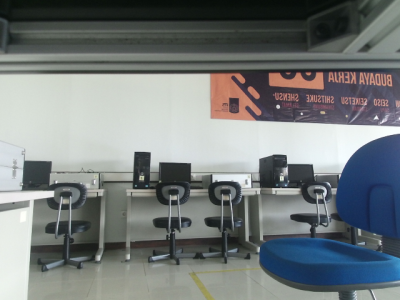
\includegraphics[width=0.225\textwidth]{figures/depth-camera/real-rgb.png}
    \label{fig:depthcameraresultrealrgb}
  }
  \hfil
  \subfloat[\IfLanguageName{english}{Depth image}{Citra kedalaman}]{
    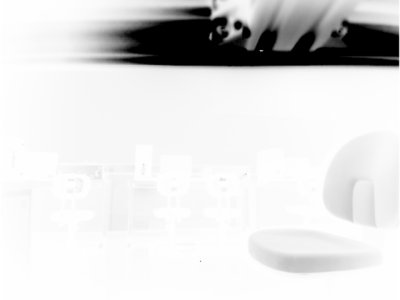
\includegraphics[width=0.225\textwidth]{figures/depth-camera/real-depth.png}
    \label{fig:depthcameraresultrealdepth}
  }
  \IfLanguageName{english}{
    \caption{Comparison of color image and depth image capture results from depth camera on the real robot.}
  }{
    \caption{Perbandingan hasil tangkapan citra warna dan citra kedalaman dari \emph{depth camera} pada robot fisik.}
  }
  \label{fig:depthcameraresultreal}
\end{figure}
